\documentclass{article}
\usepackage{graphicx}
\usepackage{listings}
\usepackage[margin=0.8in]{geometry}
\usepackage{placeins}

\title{Description and Summarization}
\author{Andrew Smith, Kofi Otseidu, Manav Trivedi}


\begin{document}
\maketitle

\section{Average Salary per District}

\begin{lstlisting}[frame=single]
COPY(SELECT dpu.unit_name,dpu.description, 
to_char(AVG(ds.salary),'99999999999999999D99') AS average_salary,
to_char(STDDEV(ds.salary),'99999999999999999D99') AS std_salary
FROM data_salary ds, data_officerhistory doh, data_policeunit dpu
WHERE dpu.id=doh.unit_id AND doh.officer_id=ds.officer_id
GROUP BY dpu.unit_name,dpu.description
ORDER BY dpu.unit_name)
TO '/tmp/output.csv' CSV HEADER;
\end{lstlisting}
\begin{center} Output- there are a lot more rows we didn't include but are output by the query
\end{center}
\begin{table}[h]
\centering
\begin{tabular}{|l|l|l|l|}
\hline
unit\_name & description                             & average\_salary & std\_salary \\
\hline
1          & District 001                            & 79064.02        & 17978.26    \\
2          & District 002                            & 77256.34        & 15402.32    \\
3          & District 003                            & 76162.29        & 16194.95    \\
4          & District 004                            & 76735.87        & 16658.48    \\
5          & District 005                            & 77075.2         & 16487.53    \\
6          & District 006                            & 76741.03        & 16712.11    \\
7          & District 007                            & 76400.79        & 16155.5     \\
8          & District 008                            & 76959.9         & 15792.98    \\
9          & District 009                            & 77530.3         & 15993.72    \\
10         & District 010                            & 77545.42        & 16779.81    \\
11         & District 011                            & 77907.7         & 17523.12    \\
12         & District 012                            & 78320.26        & 16878.12    \\
13         & District 013                            & 79438.15        & 17785.32    \\
14         & District 014                            & 78479.82        & 16597.87    \\
15         & District 015                            & 77536.95        & 16772.95    \\
16         & District 016                            & 77774.94        & 15479.94    \\
17         & District 017                            & 78412.75        & 16174.04    \\
18         & District 018                            & 77907.07        & 16258.87    \\
19         & District 019                            & 77020.29        & 15432.97    \\
20         & District 020                            & 78697.35        & 17058.13    \\
21         & District 021                            & 78697.72        & 16257.21    \\
22         & District 022                            & 77499.63        & 14673.31    \\
23         & District 023                            & 78217.89        & 15900       \\
24         & District 024                            & 78099.61        & 16276.85    \\
25         & District 025                            & 77315.81        & 16729.37    \\
26         & Executive Officers Unit                 & 107119.46       & 35073.21    \\

55         & Mounted Unit                            & 80333.32        & 15857.89   
\\
\hline
\end{tabular}
\end{table}

From the salary table, we can see that most districts are about the same. The average is roughly 77k, with some districts a bit higher and some lower. It would be interesting to compare to the civilian median income for each district. It is also interesting to look at the other units, i.e. the Mounted Unit or Bomb Squad. We had initially guessed that police officer pay would be higher in nicer neighborhoods, but for the most part it's the same across the board. This kind of makes logical sense, as having the pay higher in certain areas of the city would incentivize officers to move around. In this way, most neighborhoods would get officers of the same quality (for the most part). On some level we would almost expect officers to be paid more to police more 'dangerous' districts, but we also don't see this. I would be interested in learning why this isn't the case, but in some respects I imagine it might be a budget issue.

\FloatBarrier
\section{Allegations per District}

\begin{center}
Code
\end{center}
\begin{lstlisting}[frame=single]
COPY(
SELECT da.name, COUNT(DISTINCT dal.crid) AS num_allegations
FROM data_area da, data_allegation dal
WHERE da.area_type='police-districts' AND ST_Intersects(dal.point,da.polygon)
GROUP BY da.name
ORDER BY num_allegations DESC)
TO '/tmp/allegations.csv' CSV HEADER;
\end{lstlisting}


\begin{table}[h]
\centering
\begin{tabular}{|l|l|}
\hline
District Name & num\_allegations \\
\hline
1st  & 10721            \\
11th & 10009            \\
8th  & 9172             \\
7th  & 8993             \\
9th  & 8945             \\
12th & 8465             \\
2nd  & 8072             \\
6th  & 7862             \\
4th  & 7836             \\
19th & 7020             \\
18th & 6672             \\
5th  & 6659             \\
3rd  & 6650             \\
25th & 6458             \\
10th & 6101             \\
14th & 5394             \\
15th & 5289             \\
22nd & 4910             \\
16th & 4274             \\
24th & 4181             \\
17th & 3180             \\
20th & 2876             \\
31st & 108      \\
\hline      
\end{tabular}
\end{table}

The allegations table shows that a few districts, namely the 1st and 11th, have quite a bit more allegations than the other districts. The Loop is an extremely busy area for both tourists and commuters heading to work, leading to lots of police interactions. The next few districts are in rougher neighborhoods, where again we'd expect to see more police actions and thus more complaints. These are also majority minority neighborhoods, so it's possible this plays a part in the high number of complaints.

Note: Some of the allegations are locationless. I'm not entirely sure how to handle these going forward, it may be better to do what we were doing initially, and try to trace the current officer district at the incident date.


\FloatBarrier
\section{Complaint and Resignation Dates}

\begin{center}
Code
\end{center} 
\begin{lstlisting}[frame=single]
COPY(SELECT dof.id, dof.first_name, dof.last_name, da.incident_date, 
dof.resignation_date, 
EXTRACT(day FROM COALESCE(dof.resignation_date,'2018-10-22') - da.incident_date) 
	AS days_between
FROM data_officer dof, data_officerallegation doa, data_allegation da
WHERE dof.id = doa.officer_id AND doa.allegation_id=da.id
ORDER BY dof.id)
TO '/tmp/output.csv' CSV HEADER;
\end{lstlisting}

\begin{center}
Output (first few lines)
\end{center}
\begin{table}[h!]
\begin{tabular}{|l|l|l|l|l|l|}
\hline
id & first\_name & last\_name & incident\_date         & resignation\_date & days\_between \\
\hline
4  & Carmel      & Abbate     & 1992-02-10 18:00:00-06 & 2003-08-15        & 4203          \\
4  & Carmel      & Abbate     & 2000-08-15 19:00:00-05 & 2003-08-15        & 1094          \\
4  & Carmel      & Abbate     & 2000-08-15 19:00:00-05 & 2003-08-15        & 1094          \\
4  & Carmel      & Abbate     & 1999-04-18 19:00:00-05 & 2003-08-15        & 1579          \\
4  & Carmel      & Abbate     & 1995-07-11 19:00:00-05 & 2003-08-15        & 2956          \\
4  & Carmel      & Abbate     & 1995-11-15 18:00:00-06 & 2003-08-15        & 2829          \\
4  & Carmel      & Abbate     & 1994-07-29 19:00:00-05 & 2003-08-15        & 3303          \\
5  & Carmen      & Abbate     & 1992-10-18 19:00:00-05 & 1993-06-04        & 228           \\
5  & Carmen      & Abbate     & 1991-10-11 19:00:00-05 & 1993-06-04        & 601           \\
5  & Carmen      & Abbate     & 1991-06-03 19:00:00-05 & 1993-06-04        & 731           \\
5  & Carmen      & Abbate     & 1992-11-01 18:00:00-06 & 1993-06-04        & 214           \\
6  & Anthony     & Abbate     & 1999-11-18 18:00:00-06 & 2009-12-22        & 3686          \\
6  & Anthony     & Abbate     & 2001-11-22 18:00:00-06 & 2009-12-22        & 2951          \\
6  & Anthony     & Abbate     & 2007-02-18 18:00:00-06 & 2009-12-22        & 1037          \\
6  & Anthony     & Abbate     & 2004-11-20 18:00:00-06 & 2009-12-22        & 1857          \\
6  & Anthony     & Abbate     & 2007-03-22 19:00:00-05 & 2009-12-22        & 1005          \\
6  & Anthony     & Abbate     & 1997-05-20 19:00:00-05 & 2009-12-22        & 4598          \\
8  & Leon        & Abbey      & 2001-04-19 19:00:00-05 & 2008-11-26        & 2777          \\
8  & Leon        & Abbey      & 2006-01-05 18:00:00-06 & 2008-11-26        & 1055          \\
9  & Michael     & Abbey      & 1989-10-01 19:00:00-05 & 1991-07-26        & 662           \\
9  & Michael     & Abbey      & 1990-03-25 18:00:00-06 & 1991-07-26        & 487           \\
9  & Michael     & Abbey      & 1989-10-05 19:00:00-05 & 1991-07-26        & 658          
\\
\hline
\end{tabular}
\end{table}

The dates table provides some interesting information, but without some more analysis it's hard to draw any conclusions. Some officers go for years after getting complaints, some resign soon. To improve upon this we would probably make a table with the date of the first complaint, last complaint, resignation date, days between each, and also number of complaints each. From there we might be able to glean more information about the correlation.

The plots below look into some of these relations. In these cases I replaced the resignation date with today's date for empty values---this may introduce some errors for officers whose resignation dates exist, but weren't recorded, so I've cut off any extreme outlier values in the plots, of which there aren't many. The first plot shows the time in days between an allegation and resignation date for an officer. This includes all complaints, so for any officer that has multiple complaints, they'll show up multiple times. The second and third are more refined, showing the time between the first complaint and last complaint, respectively. Note that the third plot includes the second plot for officers who only received one complaint. The second plot shows us that often an officer will resign shortly after their first complaint, however the third plot shows almost no relation between the dates. Cynically I would assume that it's much easier to oust a junior officer, who would be getting their first complaint. On the other hand, officers receiving a lot of complaints are probably older and higher up in the police hierarchy and thus harder to fire altogether. It would also be helpful to look into the amount of time it takes for complaints to go through the database in general. Looking at the plots, 2000 days is over 5 years, which seems like a long amount of time between the complaint and resignation, so it's hard to tell if the complaint was actually the cause. On the other hand, maybe police departments wait until a bit later to fire officers ostensibly for other transgressions.


\begin{figure}[h!]
\centering
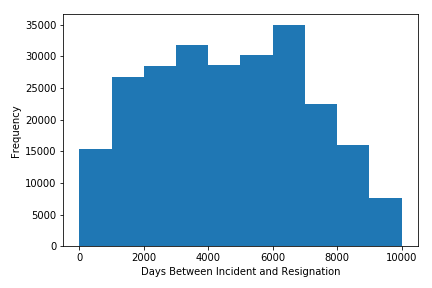
\includegraphics[width=0.5\textwidth]{complaint1.png}
\end{figure}

\begin{figure}[h!]
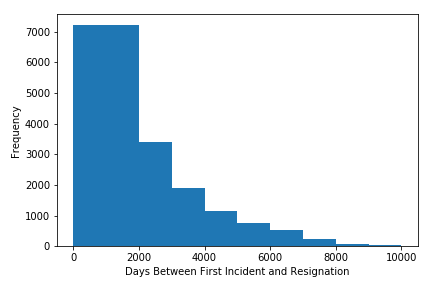
\includegraphics[width=0.5\textwidth]{complaint2.png}
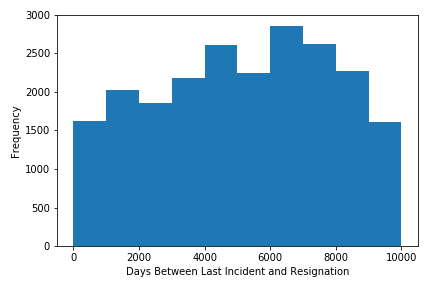
\includegraphics[width=0.5\textwidth]{complaint3.png}
\end{figure}

\FloatBarrier
\section{Average Salary by Rank}

\begin{center}
Code
\end{center} 
\begin{lstlisting}[frame=single]
SELECT ds.rank, 
 to_char(
 AVG(ds.salary), '99999999999999999D99')
 AS average_salary
FROM data_salary ds 
GROUP BY ds.rank;
\end{lstlisting}

\pagebreak
\begin{center}
Output
\end{center}
\begin{lstlisting}[frame=single]
              rank               |    average_salary     
---------------------------------+-----------------------
 Commander                       |             142260.28
 Assistant Superintendent        |             180492.00
 Deputy Chief                    |             151326.22
 Field Training Officer          |              77357.17
 Detective                       |              83630.82
 Superintendent'S Chief Of Staff |             158337.00
 Investigator                    |              68444.66
 First Deputy Superintendent     |             172056.38
 Captain                         |             135291.60
 Sergeant                        |              91771.54
 Deputy Superintendent           |             153411.11
 General Counsel                 |             143630.21
 Chief                           |             171202.08
 Civilian                        |             131037.32
 Lieutenant                      |             122029.45
 Police Officer                  |              71814.93
\end{lstlisting}

The salary by rank is straightforward, and lines up with what we know of the police department hierarchy. It is interesting to see the Assistant Superintendent as the highest paid, but it appears that the superintendent isn't on the list. The civilian
entry is probably some sort of error in the database that would be worth investigating.

\end{document}
